\documentclass{article}

\usepackage{float}
% \usepackage{floatrow}
\usepackage[T1, T2A]{fontenc}
\usepackage[english, serbian c]{babel}
\usepackage[utf8]{inputenc}
\usepackage{xcolor}
\usepackage{fancyhdr}

\usepackage[a4paper, total={6in, 8in}]{geometry}

\usepackage{amsmath}
\usepackage{graphicx}
\usepackage[colorlinks=true, allcolors=blue]{hyperref}

\usepackage{hyperref}
\hypersetup{colorlinks,linkcolor={black},citecolor={blue},urlcolor={blue}}  

\title{\textbf{ИНФОРМАЦИОНИ СИСТЕМИ} \\
\vspace{10}
\Large{\textbf{АЕРОДРОМ}}}
\author{\\Тамара Ђукић, 1051/2023 \\ \textit{mi231051@alas.matf.bg.ac.rs} \\\\
        Тамара Јевтимијевић, 1045/2023 \\ \textit{mi231045@alas.matf.bg.ac.rs} \\\\
        Милош Милаковић, 1052/2021 \\ \textit{mi211052@alas.matf.bg.ac.rs} \\\\\\
        \textit{професор:} др Саша Малков \\
        \textit{асистент:} Дара Милојковић \\\\\\}

\date{Београд 2023.}

\begin{document}

\maketitle
\thispagestyle{empty} 

\vspace{17}
\begin{figure}[h!]
    \centering
    \includegraphics[width=4cm, height=4cm]{grb.png}
\end{figure} 

\newpage
\tableofcontents

\newpage
\section{Увод}
Овај рад представља пројекат из предмета \textit{Информациони системи} на мастер студијама Математичког факултета, Универзитета у Београду. Рад описује информациони систем аеродрома. 
 Свесни смо да у данашњем времену, много људи на дневном нивоу користи аеродроме, па је у складу са тим потребно да сваки аеродром има систем који савршено ради у сваком моменту. На пример, што се тиче наше домаће авио-компаније, Air Serbia је у првих шест месеци обавила 63\% више летова и превезла 87\% више путника него за исти период 2022. године \cite{bbc_srbija}. \\ 
 Дакле, наша идеја је да развијемо систем, који ће се користити приликом рада аеродрома.\\
У оквиру анализе система препознати су основни процеси и учесници у систему. За израду дијаграма у оквиру пројекта коришћени су следећи алати:
\begin{itemize}
    \item Visual Paradigm
\end{itemize}

\section{Анализа система}

\subsection{Функционисање аеродрома}
Информациони систем, који развијамо, развијамо за потребе аеродрома. На аеродрому постоје две главне групе људи, а то су путници и радници. Како функционише аеродром? Путник дође на аеродром, чекира се, преда свој пртљаг и оде на гејт да чека укрцавање. То звучи једноставно, али иза свега тога постоји један дугачак процес. Да би путник уопште могао да лети, потребан је авион. Да би авион постојао потребно је да постоји авио-компанија, која поседује тај авион и која има уговор са аеродромом. Под уговором са аеродромом, подразумева се то да авио-компанија може да користи тј. да резервише писту аеродрома и да је користи за полетање и слетање својих авиона. Даље да би ти авиони били савршено исправни у сваком моменту потребно је да постоје људи који ће одржавати и контролисати те авионе. Затим да би авиони безбедно летели постоје људи који ће их пратити и усмеравати, итд. Као што видимо систем једног аеродрома је веома комплексан и компликован. На све то, у сваком моменту, мора савршено да функционише. \\
    На слици \ref{fig:uc_diagram} налази се дијаграм, који приказује учеснике система и њихове послове.

\subsection{Учесници у систему}
Основна подела учесника је на \textbf{путнике, запослене и авио-компаније}.\\
Запослени на аеродрому:
\begin{itemize}
    \item Администратор - има улогу да одржава базу података
        \begin{itemize}
            \item Администратор задужен за резервацију писте;
            \item Администратор задужен за уношење и брисање запослених;
            \item Администратор задужен за уношење и брисање авио-компанија;
            \item Администратор задужен за захтеве авио-компанија за поправке/одржавање авиона;
            \item Администратор задужен за комуникацију са контролом лета.
        \end{itemize}
    \item Авио-механичар - задужен за поправку, проверу и одржавање авиона;
    \item Службеник - задужен за опслуживање путника;
    \item Контролор лета - задужен за праћење и навигирање авиона.
\end{itemize}

На наредној слици је приказан дијаграм контекста који описује све актере система.

\begin{figure}[H]
    \begin{center}
        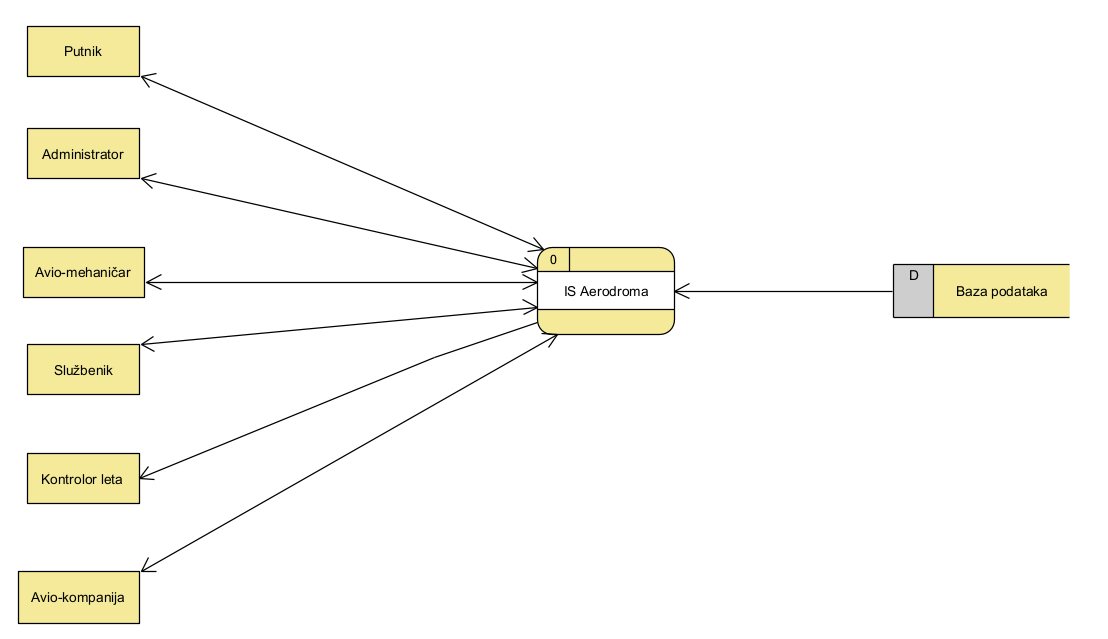
\includegraphics[width=1.1\textwidth, height=12cm]{Dijagrami_slike/dijagram_konteksta.png}
       \caption{Дијаграм контекста}
    \end{center}
\end{figure}


\subsection{Коришћени дијаграми и алати}
Током израде рада коришћени су следећи дијаграми:
\begin{itemize}
    \item UML дијаграми:
        \begin{enumerate}
            \item Дијаграм случајева употребе;
            \item Дијаграм активности;
            % \item Дијаграм секвенци.
        \end{enumerate}
    \item BPMN дијаграми ($Business$ $Process$ $Modeling$ $Notation$ $Diagram$);
    \item DFD дијаграм контекста;
    % \item ER дијаграм ($Entity$ $Relation$ $Diagram$);
    % \item Дијаграми за приказ архитектуре система;
    % \item Скице корисночног интерфејса.
\end{itemize}

За израду свих UML дијаграма
%, као и ER и BPMN дијаграма 
коришћен је алат 
\textit{Visual Paradigm - Online/Community Edition} \cite{vs}.\\\\
% За израду скица корисночног интерфејса коришћен је алат $Diagrams.net$.

\section{Процеси и случајеви употребе}

\begin{figure}[H]
\centering
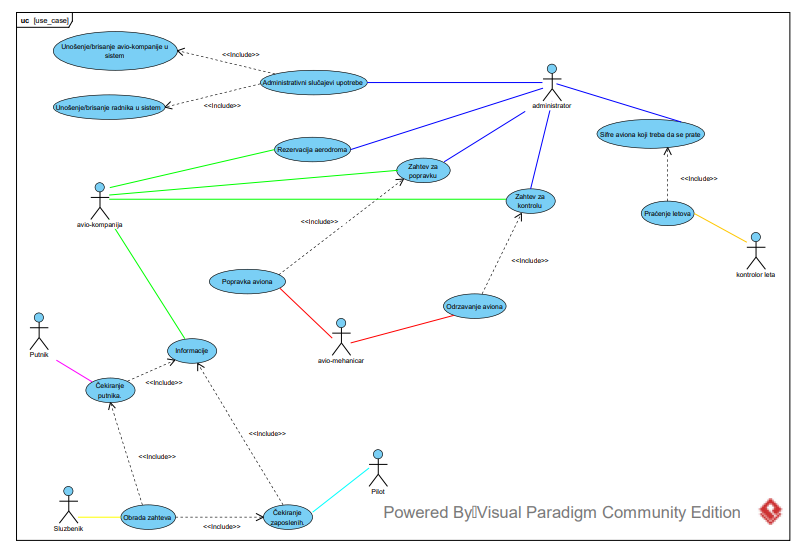
\includegraphics[width=0.9\textwidth, height=12cm]{Dijagrami_slike/uc_diagram.png}
\caption{\label{fig:uc_diagram}Дијаграм случајева употребе}
\end{figure}

\subsection{Административни случајеви употребе}

\subsubsection{Уношење радника у систем}

\begin{itemize}
    \item \textbf{Кратак опис:} Администратор уноси информације о новом раднику који у моменту уноса не постоји у систему. Систем прихвата информације и валидира их и враћа потврду о успеху или неуспеху уноса.
    \item \textbf{Учесници:}
        \begin{itemize}
            \item \textit{Администратор}
        \end{itemize}
    \item \textbf{Предуслови:} Администратор има приступ систему и има информације о раднику ког уноси.
    \item \textbf{Постуслови:} Радник је успешно додат у систем.
    \item \textbf{Основни ток:}
        \begin{enumerate}
            \item Администратор приступа систему и започиње поступак уноса радника у систем тако што отвори формулар.
            \item Систем приказује форму за унос података.
            \item Администратор уноси све потребне информације у формулар.
            \item Администратор потврђује унос.
            \item Систем валидира унете податке.
            \item Систем уноси податке у базу података.
            \item Систем обавештава администратора да је операција успешно извршена.
        \end{enumerate}
    
    \item \textbf{Алтернативни токови:}
    \item А1. \textbf{Администратор одустаје од уноса података.} Ако у кораку 4 администратор кликне на дугме одустани подаци се не шаљу систему и неће бити унети у исти.
    \item A2. \textbf{Унети подаци о раднику нису исправни.} Ако у кораку 5 систем препозна да су неки од унетих података невалидни, избациће грешку и обавестити администратора које поље је невалидно. Администратор исправља грешку и наставља даље од 4. корака главног тока. 
\end{itemize}

\begin{figure}[H]
    \centering
    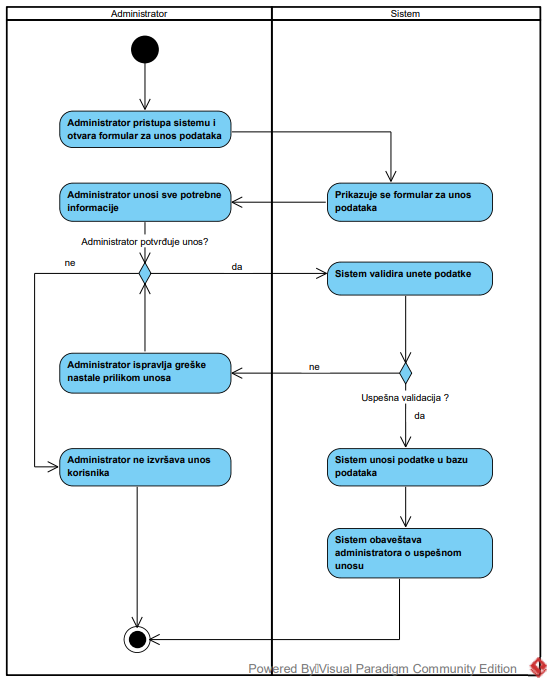
\includegraphics[width=1.1\textwidth, height=15cm]{Dijagrami_slike/dodavanje_radnika.png}
    \caption{Дијаграм активности - Додавање радника у систем}
\end{figure}

\newpage
\subsubsection{Брисање радника из система}

\begin{itemize}
    \item \textbf{Кратак опис:} Администратор брише радника који постоји у систему. Систем ажурира базу и враћа информацију о успешности захтева.
    \item \textbf{Учесници:}
        \begin{itemize}
            \item \textit{Администратор}
        \end{itemize}
    \item \textbf{Предуслови:} Администратор има приступ систему и има информације о раднику ког жели да обрише.
    \item \textbf{Постуслови:} Радник је успешно обрисан из система.
    \item \textbf{Основни ток:}
        \begin{enumerate}
            \item Администратор приступа систему и отвара страну за управљање радницима.
            \item Администратор уноси вредност за критеријум претраге.
            \item Администратор кликом на дугме врши претрагу.
            \item Систем валидира унос.
            \item Систем на основу вредности за критеријум претраге филтрира раднике и враћа резултате администратору.
            \item На основу добијених радника, администратор бира одговарајућег и подноси захтев систему за брисање.
            \item Систем брише радника и ажурира базу.
            \item Систем обавештава администратора да је операција успешно извршена.
        \end{enumerate}
    
    \item \textbf{Алтернативни токови:}
        \begin{itemize}
            \item[А1.] \textbf{Администратор одустаје од уноса података.} Ако у кораку 3 или 6 администратор одустане од брисања радника, захтев се не шаље систему и радник неће бити обрисан.
            \item[A2.] \textbf{Унети подаци за филтрирање нису исправни.} Ако у кораку 4 систем препозна да је вредност за филтрирање невалидна, избациће грешку и обавестити администратора о грешци. Администратор исправља грешку и наставља даље од 3. корака главног тока. 
        \end{itemize}
\end{itemize}

\begin{figure}[H]
    \centering
    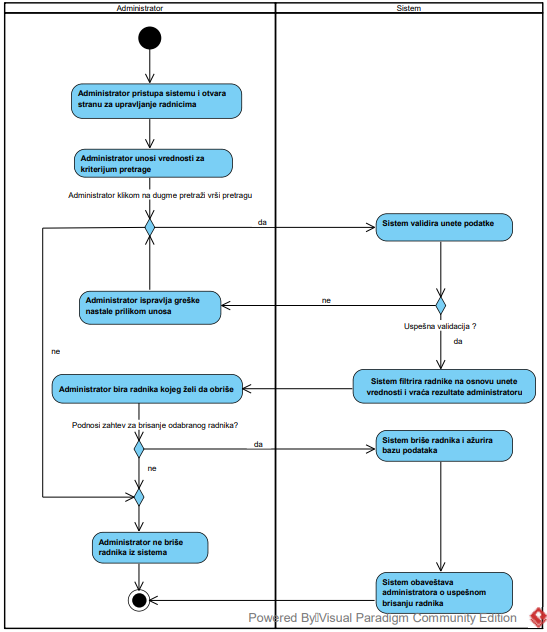
\includegraphics[width=1.1\textwidth, height=18cm]{Dijagrami_slike/brisanje_radnika.png}
    \caption{Дијаграм активности - Брисање радника из система}
\end{figure}


\subsubsection{Уношење авио-компаније у систем}

\begin{itemize}
    \item \textbf{Кратак опис:} Администратор уноси информације о новој авио-компанији која у моменту уноса не постоји у систему. Систем прихвата информације и валидира их и враћа потврду о успеху или неуспеху уноса.
    \item \textbf{Учесници:}
        \begin{itemize}
            \item \textit{Администратор}
        \end{itemize}
    \item \textbf{Предуслови:} Администратор има приступ систему и има информације о авио-компанији коју уноси.
    \item \textbf{Постуслови:} Авио-компанија је успешно додата у систем.
    \item \textbf{Основни ток:}
        \begin{enumerate}
            \item Администратор приступа систему и започиње поступак уноса авио-компаније у систем тако што отвори формулар.
            \item Систем приказује форму за унос података.
            \item Администратор уноси све потребне информације у формулар.
            \item Администратор потврђује унос.
            \item Систем валидира унете податке.
            \item Систем уноси податке у базу података.
            \item Систем обавештава администратора да је операција успешно извршена.
        \end{enumerate}
    
    \item \textbf{Алтернативни токови:}
    \item А1. \textbf{Администратор одустаје од уноса података.} Ако у кораку 4 администратор кликне на дугме одустани подаци се не шаљу систему и неће бити унети у исти.
    \item A2. \textbf{Унети подаци о авио-компанији нису исправни.} Ако у кораку 5 систем препозна да су неки од унетих података невалидни, избациће грешку и обавестити администратора које поље је невалидно. Администратор исправља грешку и наставља даље од 4. корака главног тока. 
\end{itemize}

\begin{figure}[H]
    \centering
    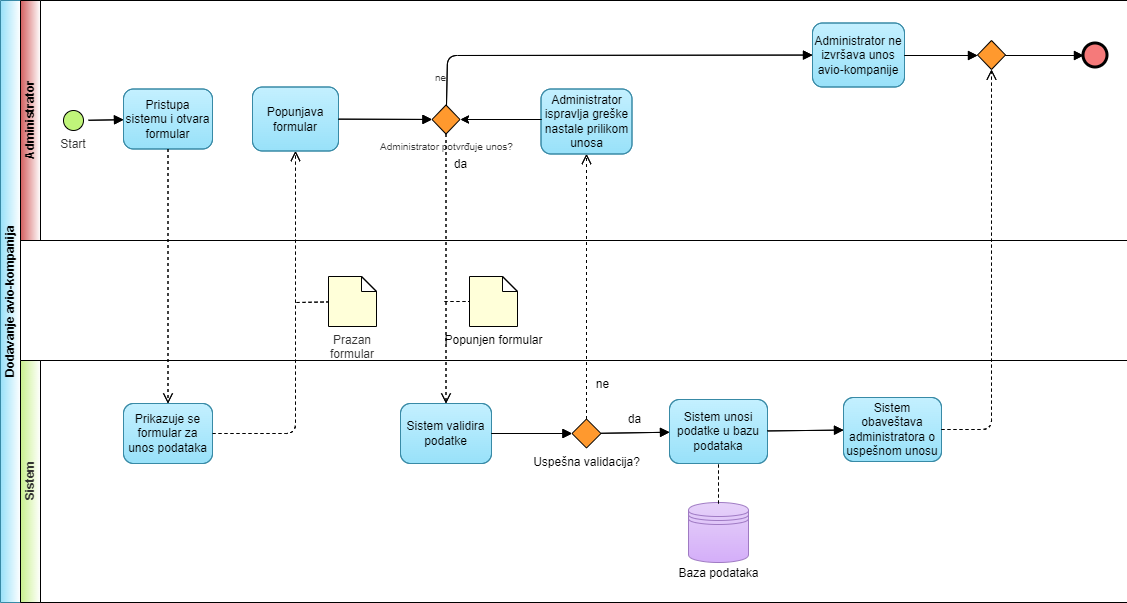
\includegraphics[width=1.1\textwidth, height=10cm]{Dijagrami_slike/dodavanje_avio_kompanije.png}
    \caption{БПМН дијаграм сарадње - Додавање авио-компаније}
\end{figure}

\newpage
\subsubsection{Брисање авио-компаније из система}

\begin{itemize}
    \item \textbf{Кратак опис:} Администратор брише авио-компанију која постоји у систему. Систем ажурира базу и враћа информацију о успешности захтева.
    \item \textbf{Учесници:}
        \begin{itemize}
            \item \textit{Администратор}
        \end{itemize}
    \item \textbf{Предуслови:} Администратор има приступ систему и има информације о авио-компанији коју жели да обрише.
    \item \textbf{Постуслови:} Авио-компанија је успешно обрисана из система.
    \item \textbf{Основни ток:}
        \begin{enumerate}
            \item Администратор приступа систему и отвара страну за управљање авио-компанијама.
            \item Администратор уноси вредност за критеријум претраге.
            \item Администратор кликом на дугме врши претрагу.
            \item Систем валидира унос.
            \item Систем на основу вредности за критеријум претраге филтрира авио-компаније и враћа резултате администратору.
            \item На основу добијених авио-компанија, администратор бира одговарајућу и подноси захтев систему за брисање.
            \item Систем брише авио-компанију и ажурира базу.
            \item Систем обавештава администратора да је операција успешно извршена.
        \end{enumerate}
    
    \item \textbf{Алтернативни токови:}
        \begin{itemize}
            \item[А1.] \textbf{Администратор одустаје од уноса података.} Ако у кораку 3 или 6 администратор одустане од брисања авио-компаније, захтев се не шаље систему и корисник неће бити обрисан.
            \item[A2.] \textbf{Унети подаци за филтрирање нису исправни.} Ако у кораку 4 систем препозна да је вредност за филтрирање невалидна, избациће грешку и обавестити администратора о грешци. Администратор исправља грешку и наставља даље од 3. корака главног тока. 
        \end{itemize}
\end{itemize}

\subsection{Резервација аеродрома (писте):}

\begin{figure}[H]
    \centering
    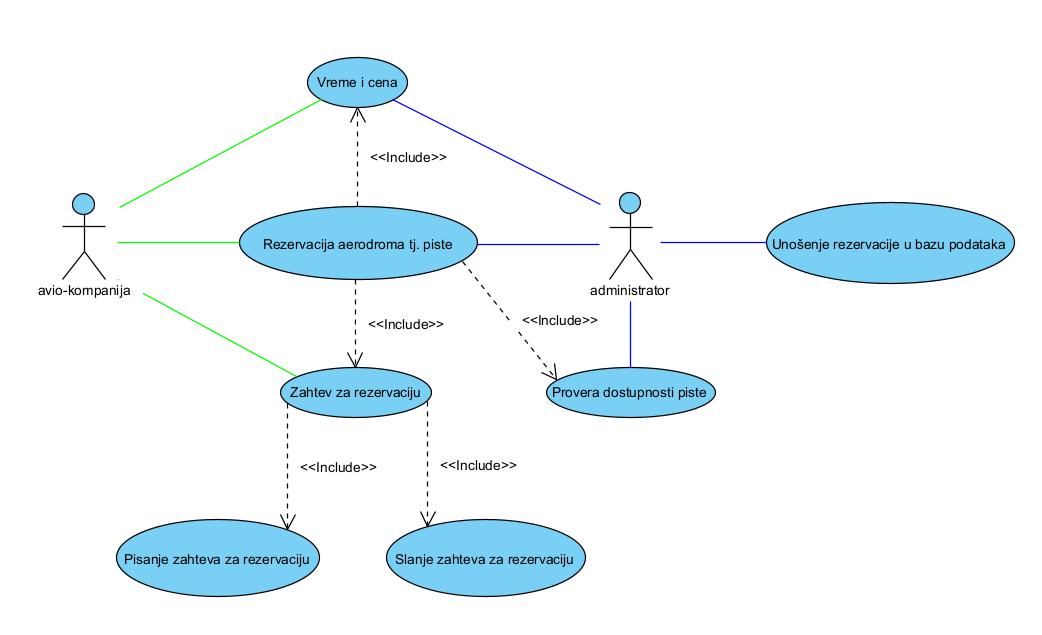
\includegraphics[width=0.9\textwidth]{Dijagrami_slike/ucs_rezervacija_aerodroma.png}
    \caption{Дијаграм случаја употребе - Резервација аеродрома (писте)}
\end{figure}

\begin{itemize}
    \item \textbf{Кратак опис:} Авио-компанија контактира са администратором аеродрома задуженим за резервације писте у циљу резервисања писте за полетање или слетање својих авиона. Са администратором може да се договара око датума, времена као и цене резервисања писте.
    \item \textbf{Учесници:}
        \begin{itemize}
            \item \textit{Авио-компанија;}
            \item \textit{Администратор који је задужен за резервације писте.}
        \end{itemize}
    \item \textbf{Предуслови:} Авио-компанија поседује барем један авион и регистрована је тј. да има уговор о пословању са аеродромом.
    \item \textbf{Постуслови:} Авио-компанија или јесте или није резервисала писту.
    \item \textbf{Основни ток:}
        \begin{enumerate}
            \item Авио-компанија пише захтев за резервацију аеродрома у ком наводи тачан датум кад жели да резервише писту.
            \item Када је написала захтев, шаље га администратору аеродрома, који је задужен за резервације писте.
            \newpage
            \item Администратор проверава доступност писте за тражени датум и проверава која времена су доступна тог датума. 
                \begin{enumerate}
                    \item Ако не постоји ниједно време у које је писта доступна тог дана:
                        \begin{itemize}
                            \item Авио-компанија отказује резервацију.
                            \item Авио-компанија мења датум и то шаље администратору.
                        \end{itemize}
                    \item Ако постоји барем једно време у које је писта слободна, администратор шаље авио-компанији цену и време могуће резервације писте.
                \end{enumerate}
            \item Авио-компанија разматра да ли цена и време одговарају или не.
                 \begin{enumerate}
                    \item Ако не одговарају, авио-компанија разматра да ли жели да откаже резервацију или не. 
                        \begin{itemize}
                            \item Авио-компанија отказује резервацију.
                            \item Авио-компанија мења датум и то шаље администратору.
                        \end{itemize}
                    \item Ако цена и време одговарају, администратор врши резервацију писте и у базу података уноси информацију о датуму, времену и ознаци авиона.
                \end{enumerate}
        \item Комуникације између администратора и авио-компаније је завршена.
    \end{enumerate}
    \item \textbf{Алтернативни токови:}
        \begin{itemize}
            \item[A1.] \textbf{Унос неисправног датума.} Уколико у кораку 2 основног тока, администратор утврди да је послат погрешан датум, авио-компанија о томе бива обавештена и процес се наставља од корака 1 основног тока.
        \end{itemize}
\end{itemize}

\newpage
\begin{figure}[H]
    \centering
    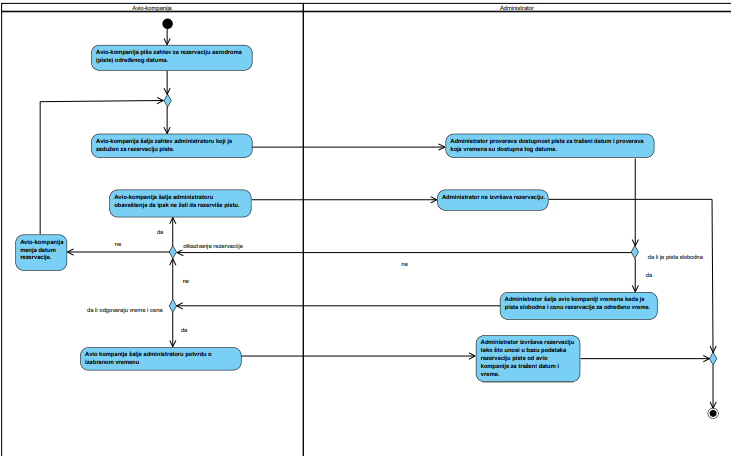
\includegraphics[width=1.1\textwidth, height=16cm]{Dijagrami_slike/rezervacija_aerodroma.png}
    \caption{Дијаграм активности - Резервација аеродрома (писте)}
\end{figure}

\newpage
\subsection{Праћење летова}

\begin{itemize}
    \item \textbf{Кратак опис:} Контролор лета прати летове тј. одређене авионе и навигира их.
    \item \textbf{Учесници:}
        \begin{itemize}
            \item \textit{Администратор}
            \item \textit{Контролор лета}
        \end{itemize}
    \item \textbf{Предуслови:} Администратор пруступа системз и има информације о шифрама авиона који лете тог дана у вадушном простору, који покрива контролни торањ или који полећу са писте. Контролор лета има комуникацију са администратором. 
    \item \textbf{Постуслови:} Контролор лета успешно комуницира са пилотима авиона и успешно их навигира и контролише.
    \item \textbf{Основни ток:}
        \begin{enumerate}
            \item Контролор лета захтева од администратора да му пошаље шифре авиона, који се налазе у ваздушном простору, који покрива торањ или који теба да полете.
            \item Администратор у најкраћем могућем року шаље потребне податке, који се аутоматки приказују на екрану испед контролора.
            \item Контролор ступа у комуникацију са пилотима авиона, које контролише, навигира их и одређује кад ко сме да слети или полети.
            \item Контролор је успешно обавио навигирање и авиони су безбедно прошли наш ваздушни простор или су безбедно слетели или полетели.
        \end{enumerate}
    
    \item \textbf{Алтернативни токови:}
        \begin{itemize}
            \item[А1.] \textbf{Авион због неких непредвиђених околности одустаје од полетања.} Ако у кораку 3 авион због неких непредвиђених околности (на пример неком је позлило и мора да дође хитна помоћ) одустао од лета, ту се основни ток, за тај конкретан лет, завршава. 
        \end{itemize}
\end{itemize}

\newpage
\subsection{Обрада захтева}

\subsubsection{Чекирање путника}

\begin{itemize}
    \item \textbf{Кратак опис:} Путник долази на шалтер аеродрома са купљеном картом, пасошем и опционо пртљагом. Службеник проверава исправност наведених докумената, и при успешној радњи, корисник добија карту за лет и иде даље на пасошку контролу.
    \item \textbf{Учесници:}
        \begin{itemize}
            \item \textit{Путник}
            \item \textit{Службеник}
            \item \textit{Авио-компанија}
        \end{itemize}
    \item \textbf{Предуслови:} Путник је купио карту (преко интернета или директно у пословници) и са пасошем и опционо пртљагом долази на аеродром.
    \item \textbf{Постуслови:} Путник се успешно чекирао на лет, добио карту и може да настави даље ка пасошкој контроли.
    \item \textbf{Основни ток:}
        \begin{enumerate}
            \item Путник на интернету или у пословници купује карту за одређени лет.
            \item Путник долази на аеродром и приступа на шалтер код службеника.
            \item Путник даје службенику пасош и уколико има пртљаг оставља га на траци.
            \item Службеник проверава пасош путника и на тај начин проверава и да ли се карта налази у бази података авио-компаније, тј. да ли путник има купљену карту.
                \begin{enumerate}
                    \item Ако се карта налази у бази података, службеник је штампа и даје је путнику.
                    \item Ако се карта не налази у бази, то значи да је путник није ни купио и он бива одбијен. 
                \end{enumerate}
            \item Ако је све исправно прошло, путник добија карту што значи да се успешно чекирао на конкретан лет.
            \item Путник наставља даље на пасошку контролу.
        \end{enumerate}
    
    \item \textbf{Алтернативни токови:}
    \begin{itemize}
        \item[А1.] \textbf{Путник одустао од лета:} Ако у кораку 2. путник из неких својих личних разлога одустане од лета основни ток се аутоматски ту завршава.
    \end{itemize}
   
\end{itemize}

\begin{figure}[H]
    \centering
    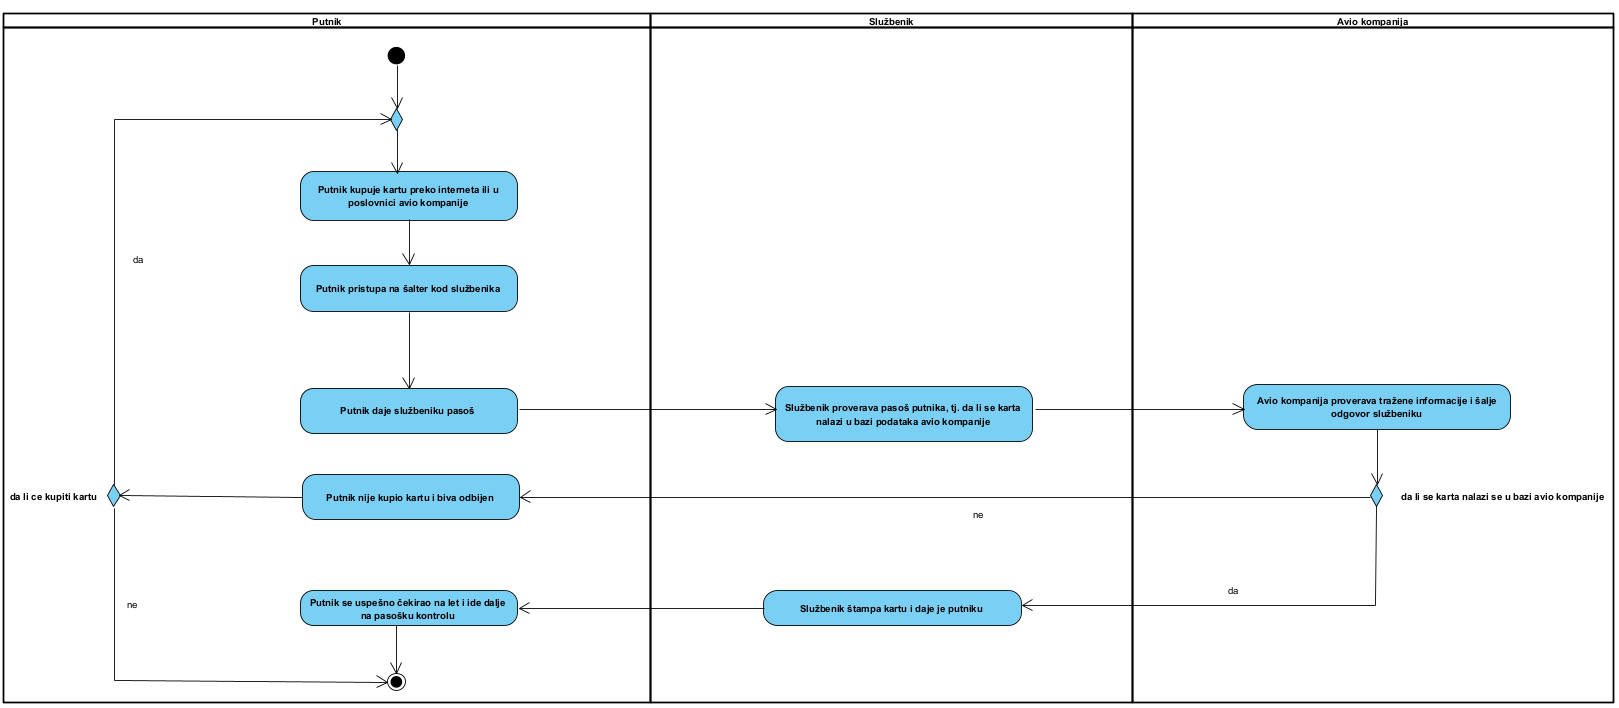
\includegraphics[width=1.1\textwidth, height=12cm]{Dijagrami_slike/cekiranje_putnika.png}
    \caption{Дијаграм случаја употребе - Чекирање путника на лет}
\end{figure}

\newpage
\subsubsection{Чекирање запослених}

\begin{itemize}
    \item \textbf{Кратак опис:} Запослен долази на шалтер аеродрома са пасошом и опционим пртљагом. Службеник проверава исправност наведених докумената, и при успешној радњи, запослен иде даље на пасошку контролу.
    \item \textbf{Учесници:}
        \begin{itemize}
            \item \textit{Запослен}
            \item \textit{Службеник}
            \item \textit{Авио-компанија}
        \end{itemize}
    \item \textbf{Предуслови:} Запослен је са пасошом и опционо пртљагом дошао на аеродром.
    \item \textbf{Постуслови:} Запослен се успешно чекирао на конкретан лет и може да настави даље ка пасошкој контроли.
    \item \textbf{Основни ток:}
        \begin{enumerate}
            \item Запослен долази на аеродром и приступа на посебан шалтер код службеника.
            \item Запослен даје службенику свој пасош.
            \item Службеник, на основу пасоша, проверава да ли се запослен налази у бази података авио-компаније и да ли је распоређен на конкретан лет.
                \begin{enumerate}
                    \item Ако је распоређен, службеник одобрава запосленом да крене даље и уноси га у систем аеродрома.
                    \item Ако није распоређен, службеник одбија запосленог и не пропушта га даље.
                \end{enumerate}
            \item Ако је све исправно прошло, запослен се успешно чекирао на конкретан лет.
            \item Запослен наставља даље ка пасошкој контроли.
        \end{enumerate}
\end{itemize}

\begin{figure}[H]
    \centering
    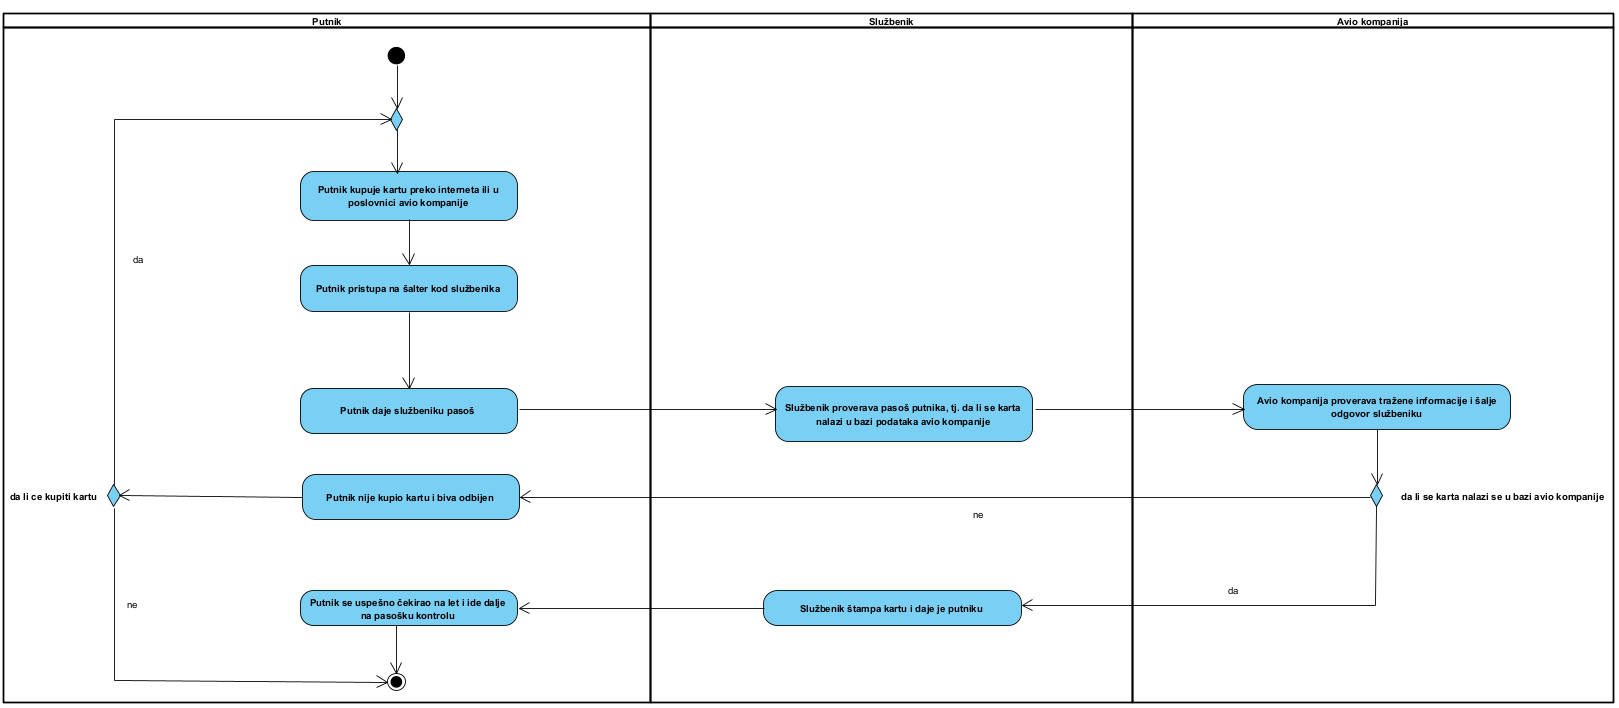
\includegraphics[width=1.1\textwidth, height=12cm]{Dijagrami_slike/cekiranje_putnika.png}
    \caption{Дијаграм случаја употребе - Чекирање запослених на лет}
\end{figure}


\newpage
\subsection{Поправка авиона}

\begin{itemize}
    \item \textbf{Кратак опис:} Авио-компанија, у тренутку квара неког авиона, захтева од аеродрома поправку конкретног авиона. Аеродром ангажује авио-механичаре, који врше целокупну поправку. Након поправке, аеродром враћа авион авио-компанији и авион је спреман за даље летење.
    \item \textbf{Учесници:}
        \begin{itemize}
            \item \textit{Авио-компанија}
            \item \textit{Администратор}
            \item \textit{Авио-механичар}
        \end{itemize}
    \item \textbf{Предуслови:} Авион кокретне авио-компаније се покварио и захтева се његова поправка. Авио-механичар (или више њих) је слободан и ангажован од стране аеродрома да поправи авион.
    \item \textbf{Постуслови:} Авио-механичар (или више њих) је успешно поправио авион, авион се враћа авио-компанији и спреман је за лет.
    \item \textbf{Основни ток:}
        \begin{enumerate}
            \item Авио-компанија је регистровала да постоји квар на конкретном авиону.
            \item Авио-компанија шаље захтев администратору администратору аеродрома за услугу поправке авиона. %  ovo treba pormeniti na dijagramu i staviti novu sliku
            \item Администратор проверава да ли има слободних авио-механичара, који ће радити на поправци авиона.
                \begin{enumerate}
                    \item Ако има слободних, авион се шаље на поправку.
                    \item Ако нема слободних, администратор обавештава авио-компанију да поправка није могућа у том тренутку.
                \end{enumerate}
            \item Механичари почињу поправку.
            \item Механичари од администратора администратора захтевају нове делове, који треба да се мењају.
                \begin{enumerate}
                    \item Ако постоје тражени делове, администратор их доставља авио-механичару.
                    \item Ако нема делове, поправка се паузира и чека се док се потребни делови не набаве.
                \end{enumerate}
            \item Након добијања делова, авио-механичари настављају поправку.
            \item Авио-механичар шаљe администратору статус поправке.
            \item Администратор затим враћа авион авио-компанији и шаље рачун за поправку/е.
        \end{enumerate}
        
        \item \textbf{Алтернативни токови:}
            \begin{itemize}
                \item[А1.] \textbf{Потребан део не може да се набави:} Ако у кораку 5. потребан део није никако могуће набавити онда се одмах прелази на корак 7.
            \end{itemize}
\end{itemize}

\begin{figure}[H]
    \begin{center}
        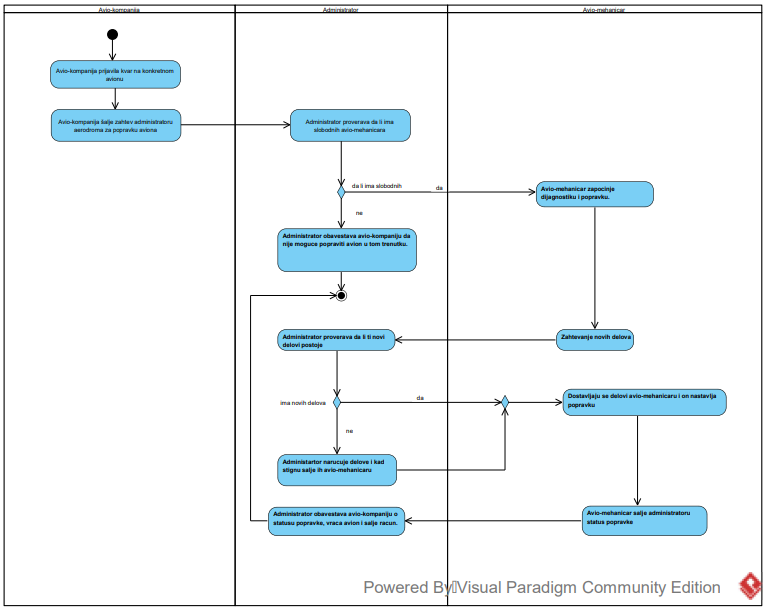
\includegraphics[width=1.1\textwidth, height=12cm]{Dijagrami_slike/popravka_aviona.png}
        \caption{Дијаграм случаја употребе - Поправка авиона}
    \end{center}
\end{figure}

\subsection{Одржавање авиона}

\begin{itemize}
    \item \textbf{Кратак опис:} Авио-компанија подноси захтев за превентивно одржавање и контролу авиона. Администратор проверава доступност механичара и ангажује их да изврше тражено одржавање.
    \item \textbf{Учесници:}
        \begin{itemize}
            \item \textit{Авио-компанија}
            \item \textit{Администратор}
            \item \textit{Авио-механичар}
        \end{itemize}
    \item \textbf{Предуслови:} Администратор има приступ систему и могућност да провери доступност авио-механичара.
    \item \textbf{Постуслови:} Авио-механичар (или више њих) је успешно одрадио одржавање авиона и извештај се подноси авио-компанији.
    \item \textbf{Основни ток:}
        \begin{enumerate}
            \item Авио-компанија подноси захтев за одржавање авиона.
            \item Администратор добија захтев.
            \item Администратор провера доступност авио-механичара.
            \item Администратор додељује одржавање авиона слободном авио-механичара.
            \item Авио-механичар врши одржавање авиона.
            \item Авио-механичар обавештава администратора о статусу авиона.
            \item Администратор отвара страну за одговор на захтев авио-компаније.
            \item Систем приказује формулар.
            \item Администратор уноси све потребне податке.
            \item Администратор потврђује унос.
            \item Систем валидира унете податке.
            \item Систем шаље авио-компанији извештај о одржавању.
        \end{enumerate}
        
    \item \textbf{Алтернативни токови:}
        \begin{itemize}
            \item[А1.] \textbf{Нема слободних авио-механичара:} Ако у 3. кораку нема доступних авио-механичара, администратор обавештава авио-компанију да тренутно не може да се одради превентивно одржавање.
            \item [A2.] \textbf{Унети подаци о одржавању авиона нису исправни:} Ако у 11. кораку систем препозна да је нека вредност у формулару невалидна, избациће грешку и обавестити администратора о грешци. Администратор исправља грешку и наставља даље од 10. корака главног тока.
        \end{itemize}
\end{itemize}

\begin{figure}[H]
    \begin{center}
        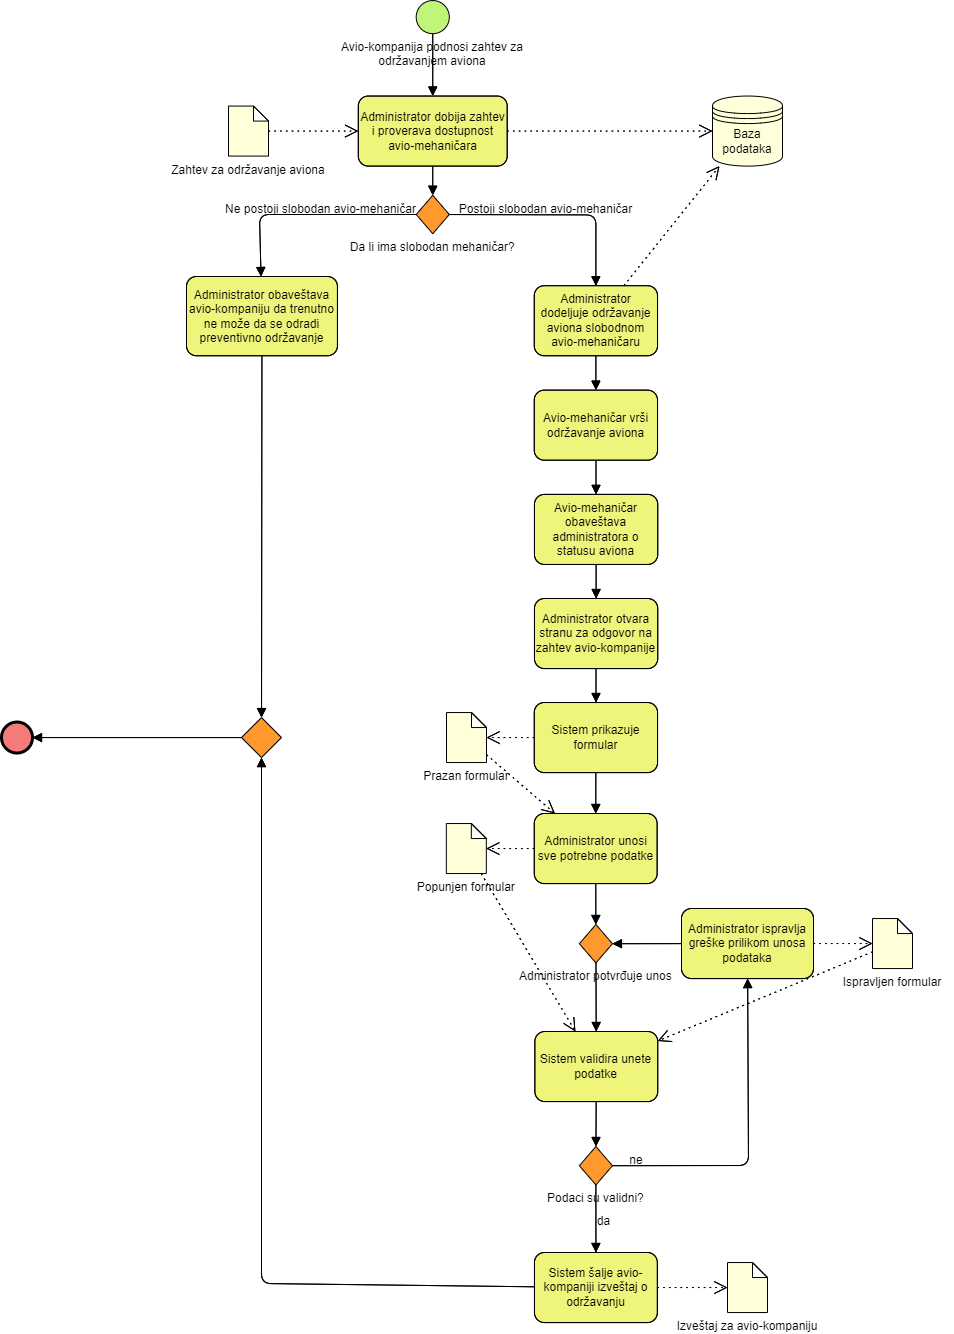
\includegraphics[width=1.1\textwidth, height=19cm]{Dijagrami_slike/odrzavanje_aviona.png}
        \caption{БПМН дијаграм процеса - Одржавање авиона}
    \end{center}
\end{figure}

\section{База података}

\section{Софтверска архитектура}

\section{Кориснички интерфејс}

\newpage
\bibliographystyle{unsrt}
\bibliography{bibliography} 


\end{document}